\chapter{16A review and prerequisites}
\section{The language of circuits}
Electrical circuits are models, specifically, abstractions of underlying physics-based descriptions of realities that govern behavior of an electrical system under analysis. Mathematically, circuits are
collections of \emph{nodes} joined by \emph{branch elements}.
Between every pair of adjacent nodes there is a \emph{voltage difference},
 measured in volts,
as well as a \emph{current}, measured in amps.
You should be able to explain, both in approximate
physical terms, and, if possible,
by a mechanical analog, what voltage and current are.
Given a circuit drawing, you should be able to write a comprehensive set
of voltage-current constraints that fully predicts what is happening
in the circuit.
For a well-posed circuit model with \(N\) nodes, one preferred method is Nodal Analysis, which involves writing \(N - 1\) linearly independent KCL node equations, and incorporating KVL and element branch consraints while writing the node equations.

\begin{figure}[H]
  \begin{center}
    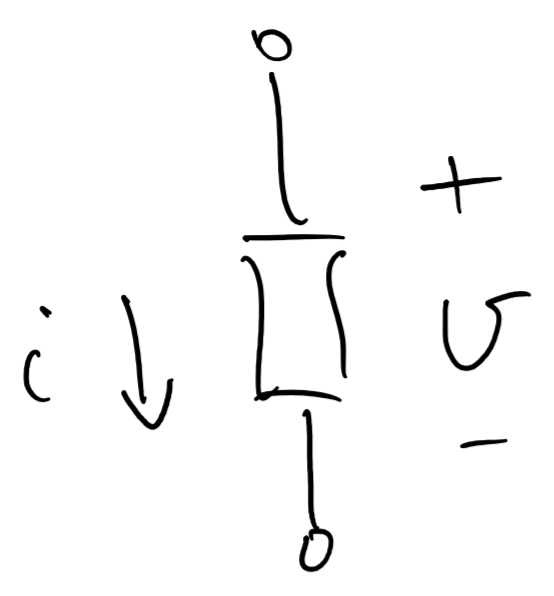
\includegraphics[width=0.25\linewidth]{figures/passive-sign}
  \end{center}
  \caption{Current and voltage annotated on a passive element.}
  \label{figure:circuit-review:passive-sign-convention}
\end{figure}
Understand how current and voltage are annotated on a circuit.
% A passive circuit element, such as a resistor, capacitor, or
% inductor\footnote{To be introduced later in 16B.}
% participates in dissipating energy from a circuit, mainly as heat.
Our terms are ``voltage \emph{across} branch element X''
and ``current \emph{through} branch element X.''
The phrases ``voltage
\emph{through}\ldots'' or ``current \emph{across}\ldots'' do not
make sense.
Understand, as shown in
Fig.~\ref{figure:circuit-review:passive-sign-convention},
that the reference directions for voltage and current are such that
% However,
% on an active circuit element, the arrow is drawn in the opposite direction.
power absorbed by a circuit element is given by
the formula \(vi\).
%\footnote{You can remember this by the Latin noun
% \emph{virtus}, which means ``strength.''}

\section{Current-voltage characteristic}
% Circuits are fully determined by their schematics because each element
% imposes a one-to-one\footnote{The assumption that
% I-V is a one-to-one correspondence
% can be relaxed in the physical world as well as in exotic exam problems,
% but only rarely.}
% constraint between its current and voltage.

\subsection{Resistor}
\begin{figure}
  \centering
  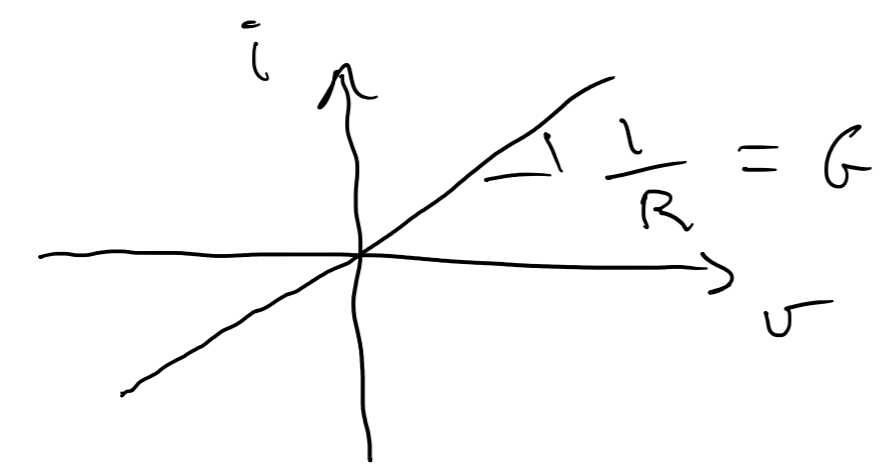
\includegraphics[width=0.5\linewidth]{figures/IV-resistor}
  \caption{I-V characteristic of a resistor.}
  \label{figure:circuit-review:IV-resistor}
\end{figure}
As shown in Fig.~\ref{figure:circuit-review:IV-resistor},
resistors enforce a proportionality relationship between
current and voltage:
\begin{align}
  V &= RI\\
  I &= GV
\end{align}
The ratio \(V/I\) is called \emph{resistance}.
The ratio \(I/V\) is called \emph{conductance}.

\subsection{Voltage source}
\begin{figure}
  \centering
  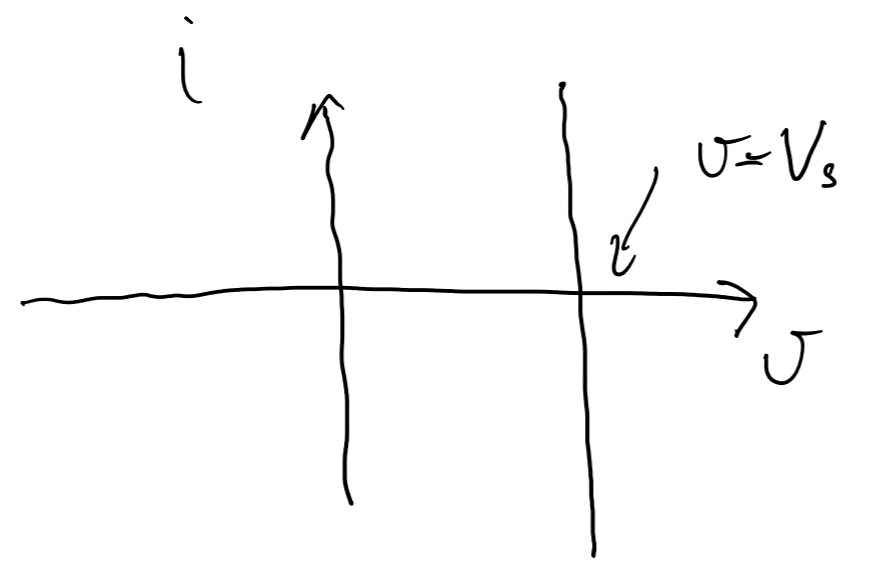
\includegraphics[width=0.5\linewidth]{figures/IV-voltage-source}
  \caption{I-V characteristic of a voltage source.}
  \label{figure:circuit-review:IV-VS}
\end{figure}
As shown in Fig.~\ref{figure:circuit-review:IV-VS},
a voltage source will provide any current (or none at all) to
maintain its target voltage.

\subsection{Current source}
\begin{figure}
  \centering
  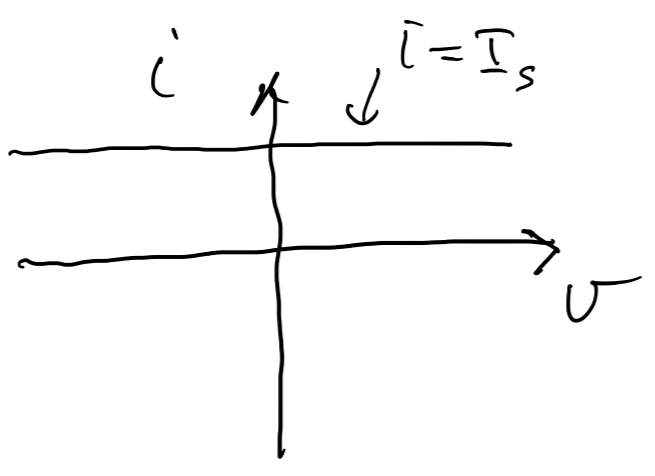
\includegraphics[width=0.4\linewidth]{figures/IV-current-source}
  \caption{I-V characteristic of a current source.}
  \label{figure:circuit-review:IV-CS}
\end{figure}
As shown in Fig.~\ref{figure:circuit-review:IV-CS},
a current source will provide any voltage (or none at all) to
maintain its target current.

\subsection{Circuit-solving techniques}
Be familiar with the following methods for solving circuits:
\begin{itemize}
  \item Series elements, e.g.~two resistors in series
  \item Parallel elements, e.g.~two resistors in parallel.
  \item Voltage and current dividers
  \item Kirchoff's voltage and current laws
  \item Norton and Th\'evenin equivalent circuits
  \item Nodal analysis
  \item Power calculations
\end{itemize}

\section{Linear algebra}
Know what a vector is. Know what eigenvalues and eigenvectors are,
and know how to solve for the eigenvalues and eigenvectors of a matrix,
by solving for the null space of \(A - \lambda I\), where
\(\lambda\) is an indeterminate. Know why this technique works.
